\subsection{Stability Analysis of the Equilibrium}
Based on the previous section, we can draw the vectors around the equilibrium as Figure \ref{fig:equilibrium_stability}.

\begin{figure}[h]
  \centering
  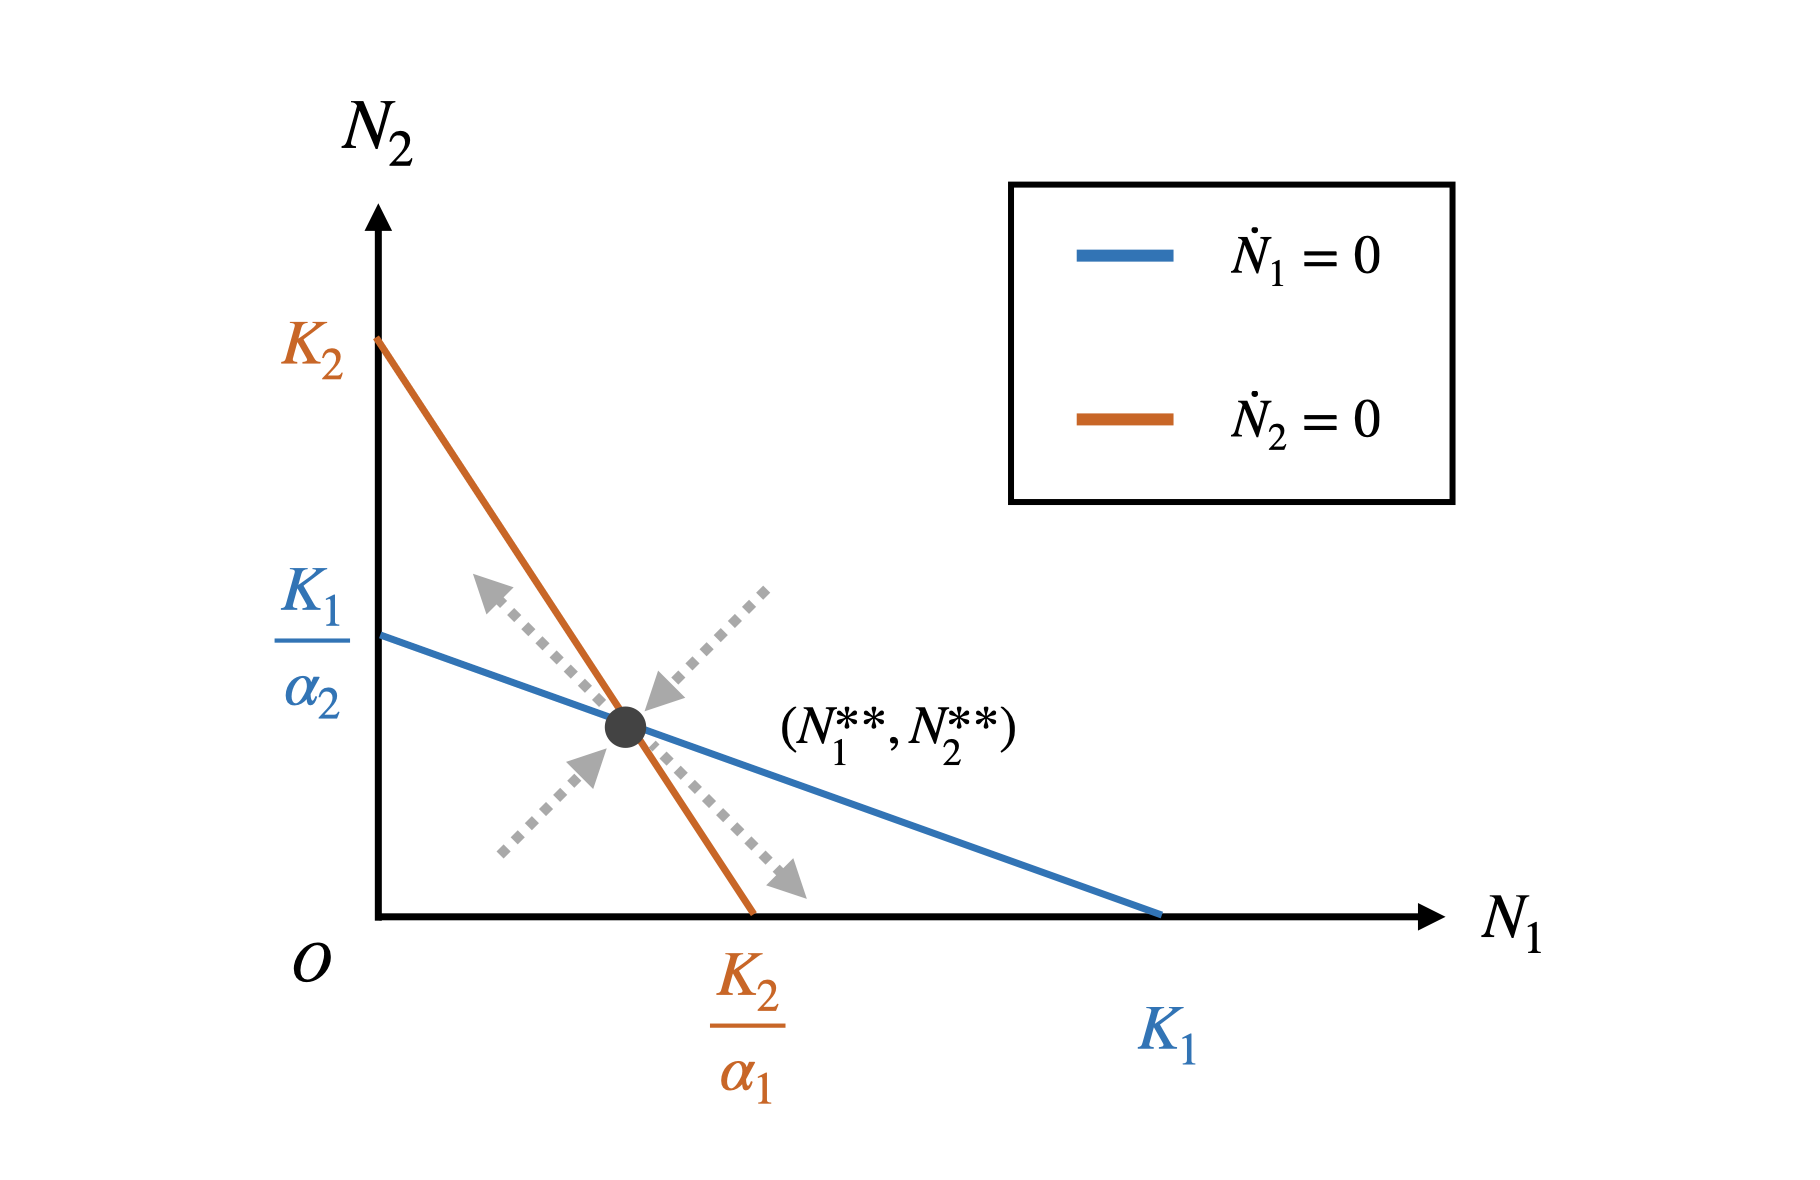
\includegraphics[width = \textwidth]{fig/graph_003.png}
  \caption {Vector space around the equilibrium in the Lotka-Volterra model when Equation \ref{equ:constraints} is met, derived from Figure \ref{fig:vecspace} . The dotted gray arrows indicate the direction of the vector after combining the previous 2 arrows.}
  \label{fig:equilibrium_stability}
\end{figure}

As we can see from the figure, the equilibrium is a saddle point, where it is stable in one axis and unstable in its orthogonal axis.
